\documentclass[10pt,a4paper]{article}
\usepackage[utf8]{inputenc}
\usepackage{amsmath}
\usepackage{amsfonts}
\usepackage{amssymb}
\usepackage{geometry}
\usepackage{verbatim}
\usepackage{enumerate}
\usepackage{fancyvrb}
\usepackage{graphicx}
\usepackage{tikz}
\usepackage{upgreek}
\usepackage{hyperref}

\usetikzlibrary{positioning}
\usetikzlibrary{shapes,snakes}
\usepackage[english]{babel}

\geometry{legalpaper, margin=1.5in}

\author{William Schultz}
\begin{document}
\title{Model Checking}
\author{William Schultz}
\maketitle

At a high level, \textit{model checking} is a computer assisted method for the analysis of dynamical systems that can be modeled as discrete state transition systems \cite{Clarke2018ch1}. In the basic setting, we can view the model checking problem as taking in a transition system (e.g. a Kripke structre) $K$ and some system specification $\upvarphi$ (typically specified in some temporal logic)  and verifying whether 
\begin{align*}
    K \vDash \upvarphi
\end{align*}
and, if $K \nvDash \upvarphi$, returning a counterexample. In the basic scenario, we can assume $K$ is finite state.

\section{Temporal Logic Model Checking}

There are a variety of temporal logics that have been used to reason about properties of programs/systems. A high level overview is shown in the relationship diagram below, where CTL* is one of the most expressive logics (encompassing both CTL and LTL).
\begin{center}
    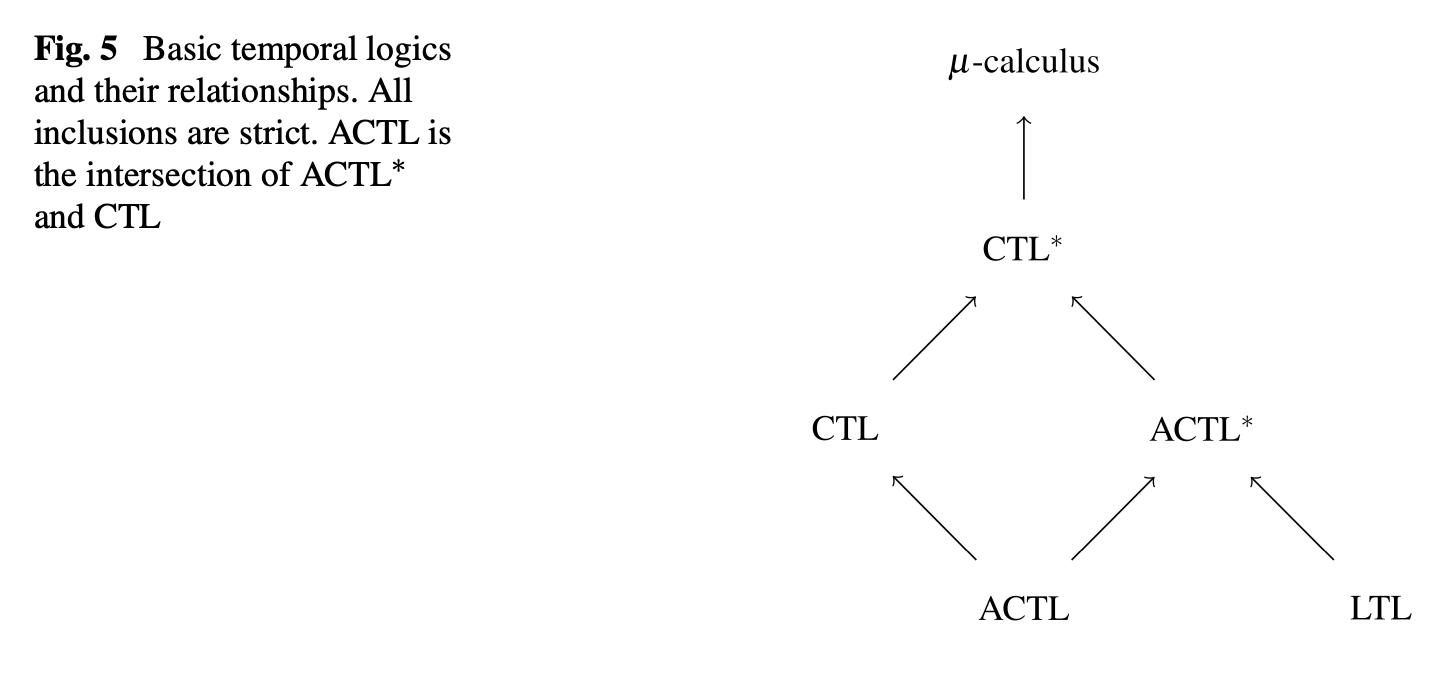
\includegraphics[scale=0.3]{images/temp-logics.png}
\end{center}
In practice, I don't think it's that important to worry much about the finer distinctions between the various logics, since typically I am more concerned with how to express a desired correctness property (e.g. for which LTL may often be sufficient). Nevertheless, it is good to have a general view of the classification hierarchy to understand the landscape (and since various papers may choose to express/formalize things in different choices of logics).

The below diagram also shows the relationship between LTL, CTL, and CTL*. Namely, that LTL and CTL are not directly comparable, and CTL* subsumes them both.
\begin{center}
    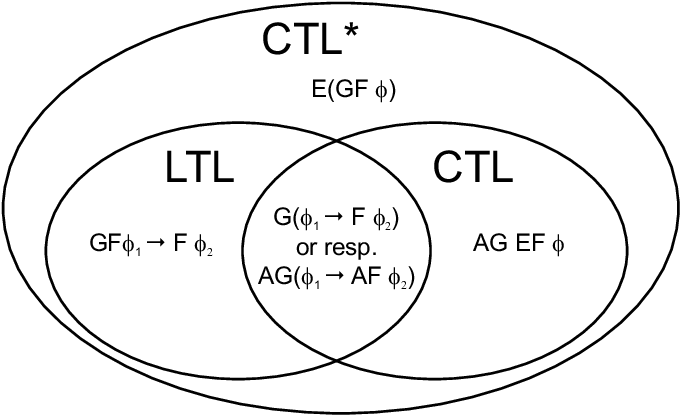
\includegraphics[scale=0.2]{images/Expressive-Power-of-LTL-CTL-and-CTL.png}   
\end{center}
The following diagram \cite{Clarke2018ch1} also provides a good overview of common varieties of temporal logic properties and their counterexample characterizations.
\begin{center}
    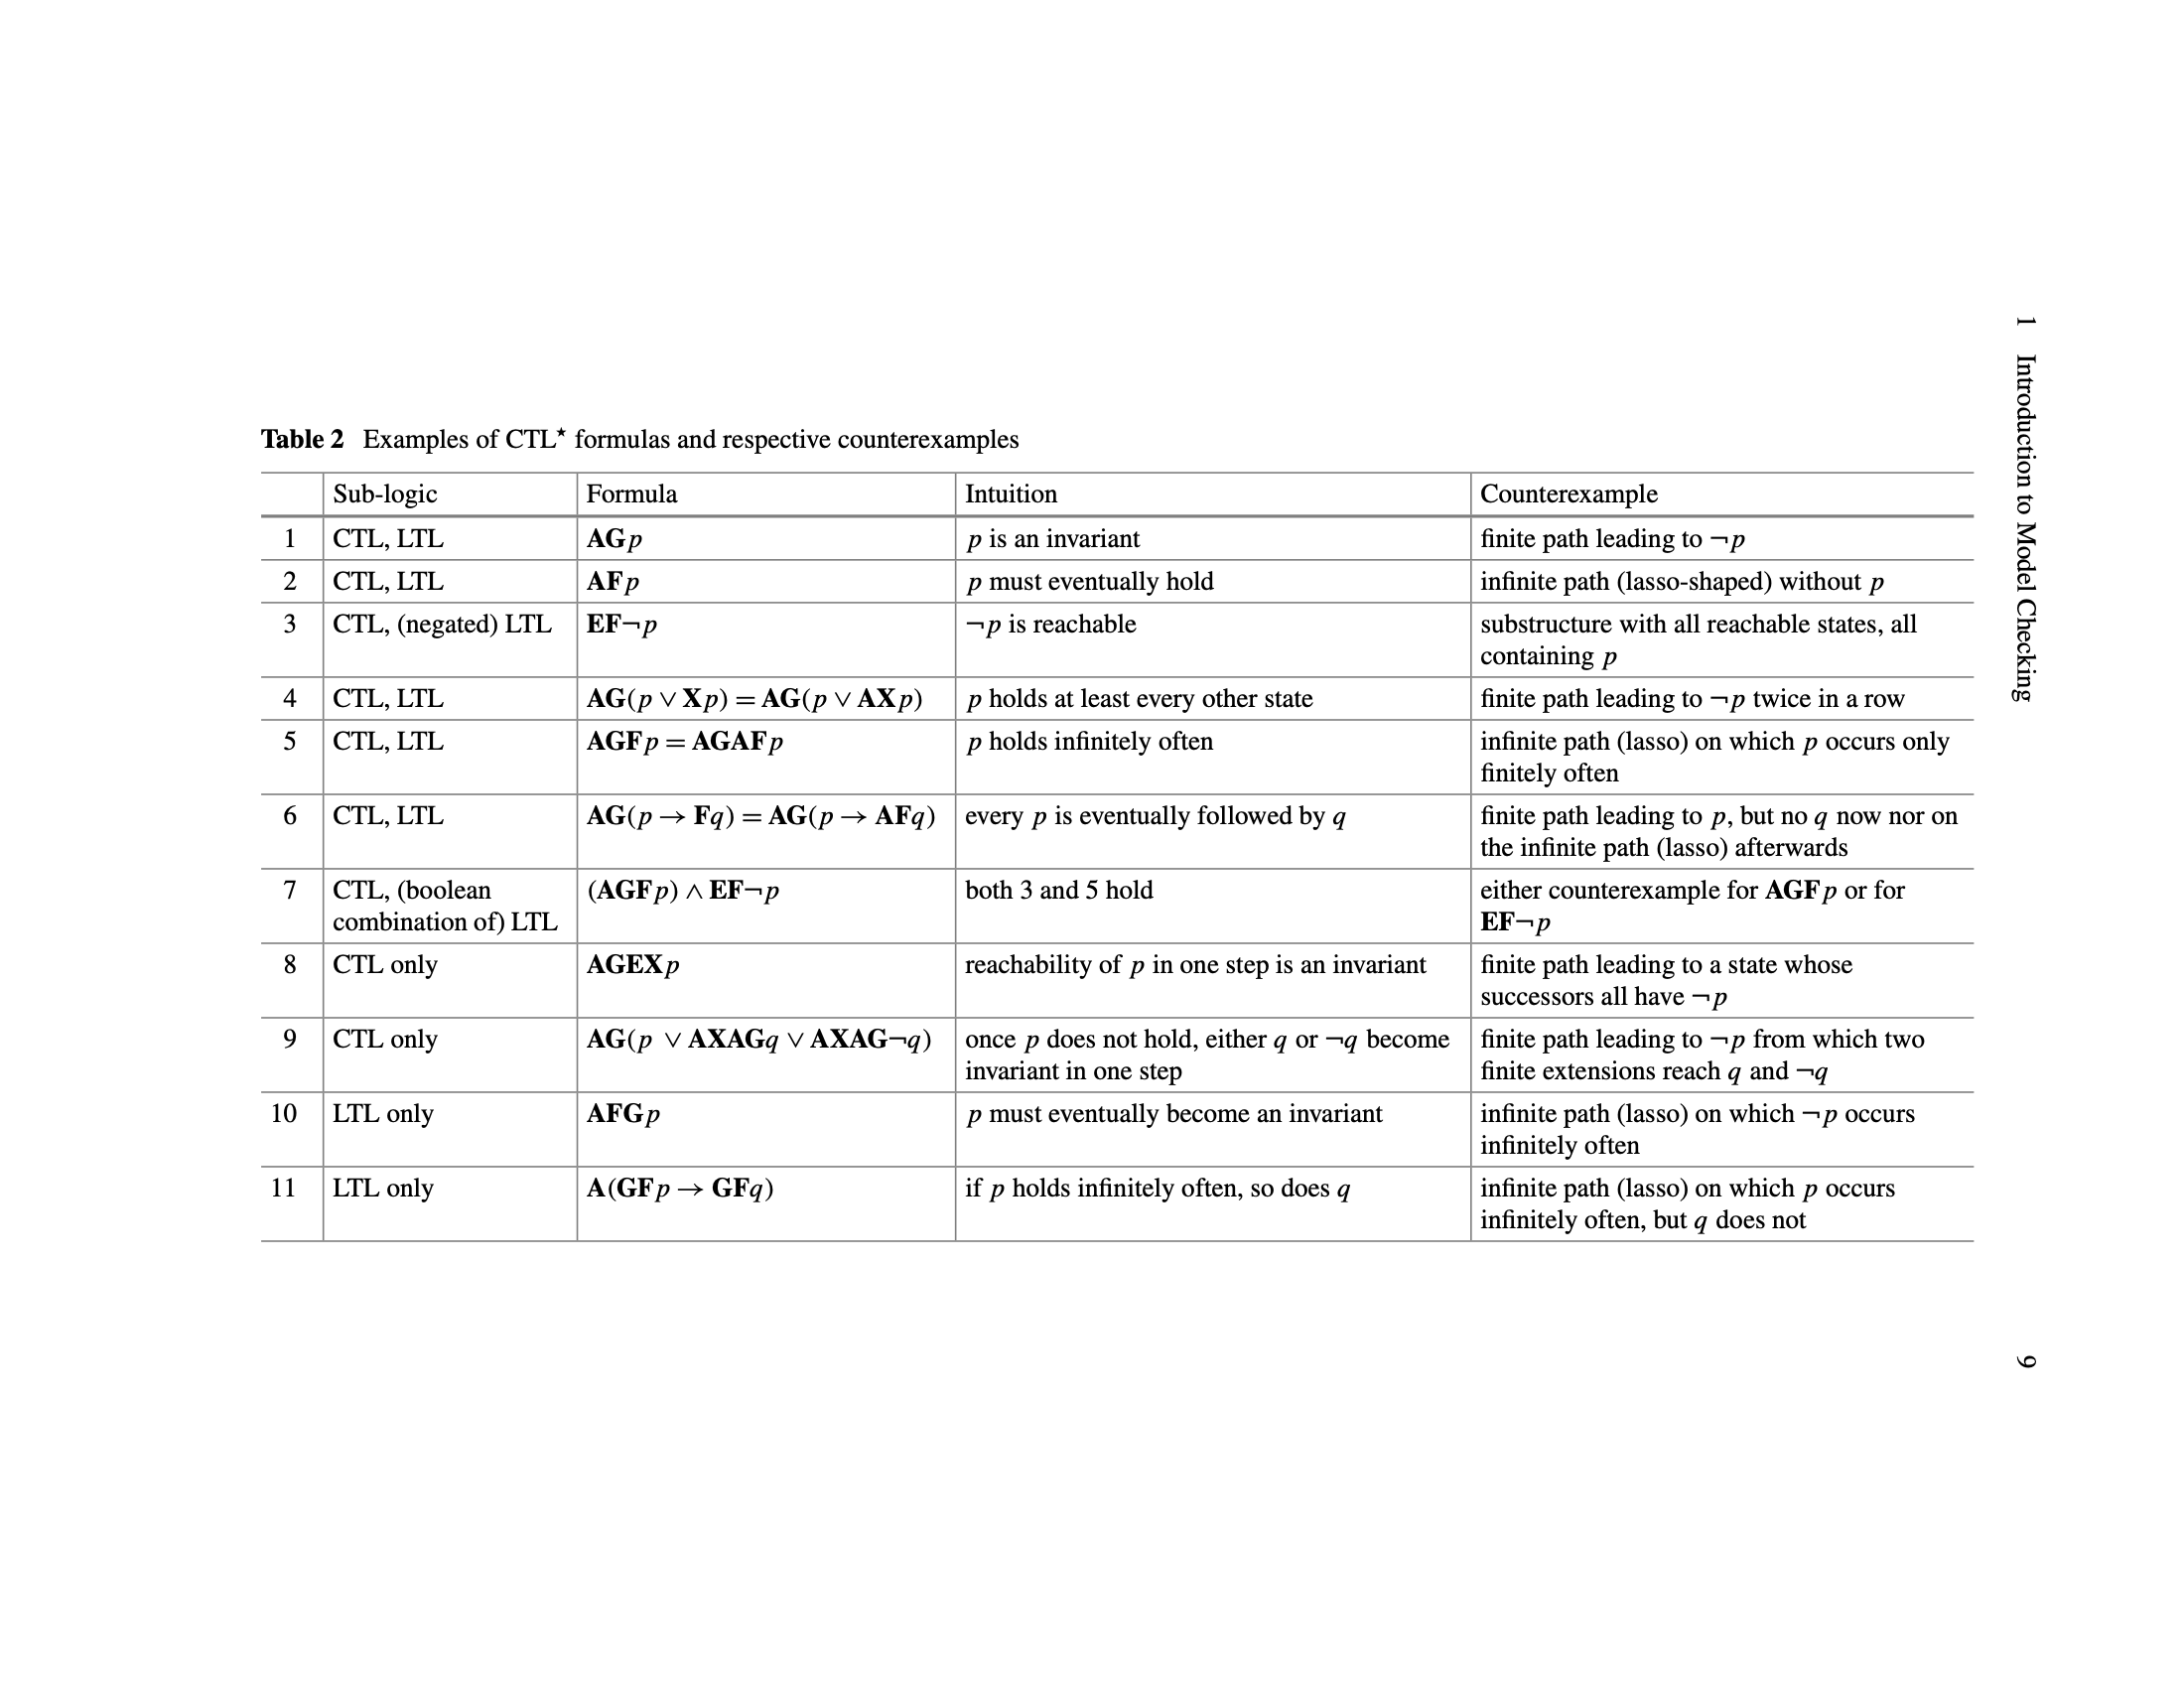
\includegraphics[scale=0.18]{images/common_ctl_ltl_formulas.png}
\end{center}

\subsection*{CTL Model Checking}

For \textit{computation tree logic} (CTL), there is a model-checking algorithm whose running time depends linearly on the size of the Kripke structure and on the length of the CTL formula \cite{1986clarkeemerson}.

\subsection*{LTL Model Checking}

For \textit{linear temporal logic} (LTL) it is the case that any counterexample to a property $\psi$ is w.l.o.g. restricted to have a ``lasso'' shape $v\cdot w^{\omega}$ i.e., an initial path (prefix) followed by an infinitely repeated finite path (cycle) \cite{1983wolpervardi}. Certain LTL properties have even simpler counterexamples e.g. safety properties always have finite paths as counterexamples. Note that the ``lasso''-ness of LTL counterexamples is exploited in certain model checking approaches e.g. some liveness to safety reductions \cite{BIERE2002160}.

\begin{center}
    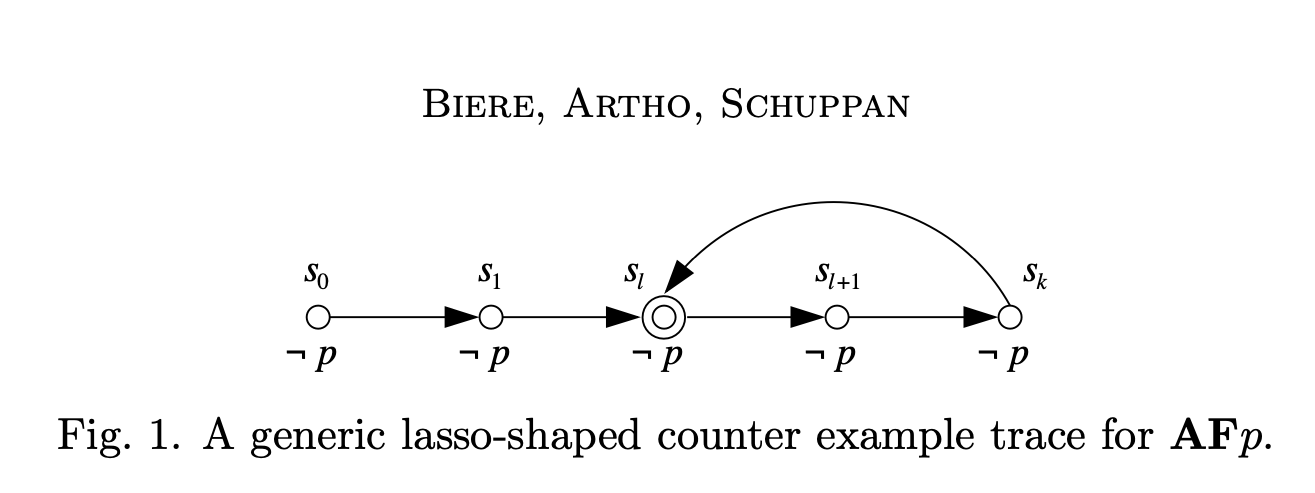
\includegraphics[scale=0.3]{images/ltl-lasso.png}
\end{center}

There is an LTL model checking algorithm whose running time depends linearly on the size of the Kripke structure and exponentially on the length of the LTL formula \cite{1985pnuelilich}. This is done by translating an LTL specification $\psi$ into a B{\"u}chi automata $B_{\psi}$ over the alphabet $2^A$ (where $A$ is the set of atomic propositions) such that for all Kripke structures $K$ and infinite paths $\pi$, the infinite word $L(\pi)$ is accepted by $B_{\psi}$ iff $\pi$ is a counterexample of $\psi$ in $K$. The size of the automaton $B_{\psi}$, though, can be exponential in the length of the formula $\psi$. 

More precisely, we translate the negation of our property $\neg \psi$ into a Buchi automaton, and then consider the product of this automaton with our original system $K \times B_{\neg \psi}$. The problem then reduces to checking whether there are any accepting runs in $K \times B_{\neg \psi}$. Recall that an accepting run in a (deterministic) Buchi automaton is any run that visits an accepting state infinitely often. A standard algorithm for checking existence of an accepting run consists of
\begin{enumerate}
    \item Consider the automaton as a directed graph and decompose it into its \href{https://will62794.github.io/my-notes/notes/Strongly_Connected_Components/Strongly_Connected_Components.html}{strongly connected components} (SCCs).
    \item Run a search to find which SCCs are reachable from the initial state
    \item Check whether there is a non-trivial SCC (i.e. consists of $\geq 1$ vertex) that is reachable and contains an accepting state.
\end{enumerate}

Technically, the LTL model checking problem is PSPACE-complete \cite{1985sistlaclarke}, but it's worth keeping in mind that in practice the limiting complexity factor is usually the size of a system's state space, rather than the size of the temporal specification. (TODO: why PSPACE?)

\subsection{Liveness to Safety Translation}

Safety checking (e.g. checking invariants) amounts to reachability analysis on the state graph of a transition system/Kripke structure. It turns out we can apply the same verification approach to liveness properties, motivated by the fact that violations to liveness properties in finite systems are \textit{lasso}-shaped i.e. they consist of a prefix that leads to a loop. The problem then becomes how to detect such a loop. In the translation given in \cite{2002bierelivenessassafety}, the loop is found by saving a previously visited state and later checking whether the current state already occurred.


\section{Abstraction for Model Checking}

Abstraction, in the context of model checking, is generally aimed at reducing the size of the state space in an attempt to remove details that are irrelevant to the property being verified \cite{Dams2018}. That is, broadly, abstraction is a fundamental tool in tackling the ``state explosion'' problem.


\subsection*{Abstraction of Kripke Structures}

In general, an abstraction framework defines a set of concrete objects and abstract objects and a definition of how to map between them. For model checking, we typically use Kripke structures as our concrete objects. Recall that a \textit{Kripe structure} $M=(AP,S,I,R,L)$ is defined as
\begin{itemize}
    \item a set $AP$ of atomic propositions
    \item a set of states $S$
    \item a set of initial states $I \subseteq S$
    \item a transition relation $R \subseteq S \times S$
    \item a labeling function $L : S \rightarrow 2^{AP}$
\end{itemize}

\subsubsection*{Simulation}
To define a notion of abstraction for Kripke structures, we define a few standard relations between two structures $M_1$ and $M_2$. \textit{Simulation} is a preorder (a reflexive and transitive partial order) in which the larger structure may have more behaviors, but possibly fewer states and transitions.

Let $M_1=(AP_1,S_1,I_1,R_1,L_1)$ and $M_2=(AP_2,S_2,I_2,R_2,L_2)$ be Kripke structures such that $AP_2 \subseteq AP_1$. A relation $H$ is a \textit{simulation relation from $M_1$ to $M_2$} if for every $s_1 \in S_1$ and $s_2 \in S_2$ such that $H(s_1,s_2)$, both of the following conditions hold:
\begin{itemize}
    \item $\forall p \in AP_2 : p \in L_1(s_1) \iff p \in L_2(s_2)$
    \item $\forall t_1 \in S_1 :  R_1(s_1,t_1) \Rightarrow \exists t_2 : (R_2(s_2,t_2) \wedge H(t_1,t_2))$
\end{itemize}
Note that it is helpful to visually illustrate these conditions e.g. if there is a (blue) transition $s_1 \rightarrow s_1'$ in system $M_1$, and states $s_1,s_2$ are related via the simulation relation $H$, then there must exist a (red) transition $s_2 \rightarrow s_2'$ such that $(s_1',s_2') \in H$.
\begin{center}
\begin{tabular}{c c c}
    $\textcolor{blue}{s_1}$ & $\overset{H}{\longrightarrow}$ & $\textcolor{red}{s_2}$ \\
    $\textcolor{blue}{\downarrow}$ &  & $\textcolor{red}{\downarrow}$ \\
    $\textcolor{blue}{s_1'}$ & $\overset{H}{\longrightarrow}$ & $\textcolor{red}{s_2'}$
    % &s_1 \longrightarrow &s_2 \\
    % &\Downarrow &\Downarrow \\
    % &s_1' \longrightarrow &s_2'
\end{tabular}
\end{center}

The second condition states that for every transition of the ``smaller'' (i.e. more concrete) system $M_1$, there must exist a corresponding transition in the larger system $M_2$. We say that $M_1$ \textit{is simulated by} $M_2$ (or $M_2$ \textit{simulates} $M_1$), denoted $M_1 \leq M_2$, if there exists a simulation relation $H$ from $M_1$ to $M_2$ such that 
\begin{align*}
    \forall s_1 \in I_1 : (\exists s_2 \in I_2 : H(s_1,s_2))
\end{align*}
For example, consider the concrete Kripke structure $M$, modeling a mutual exclusion program where its atomic propositions $AP=\{N_1,T_1,C_1,N_2,T_2,C_2,F_0\}$:
\begin{center}
    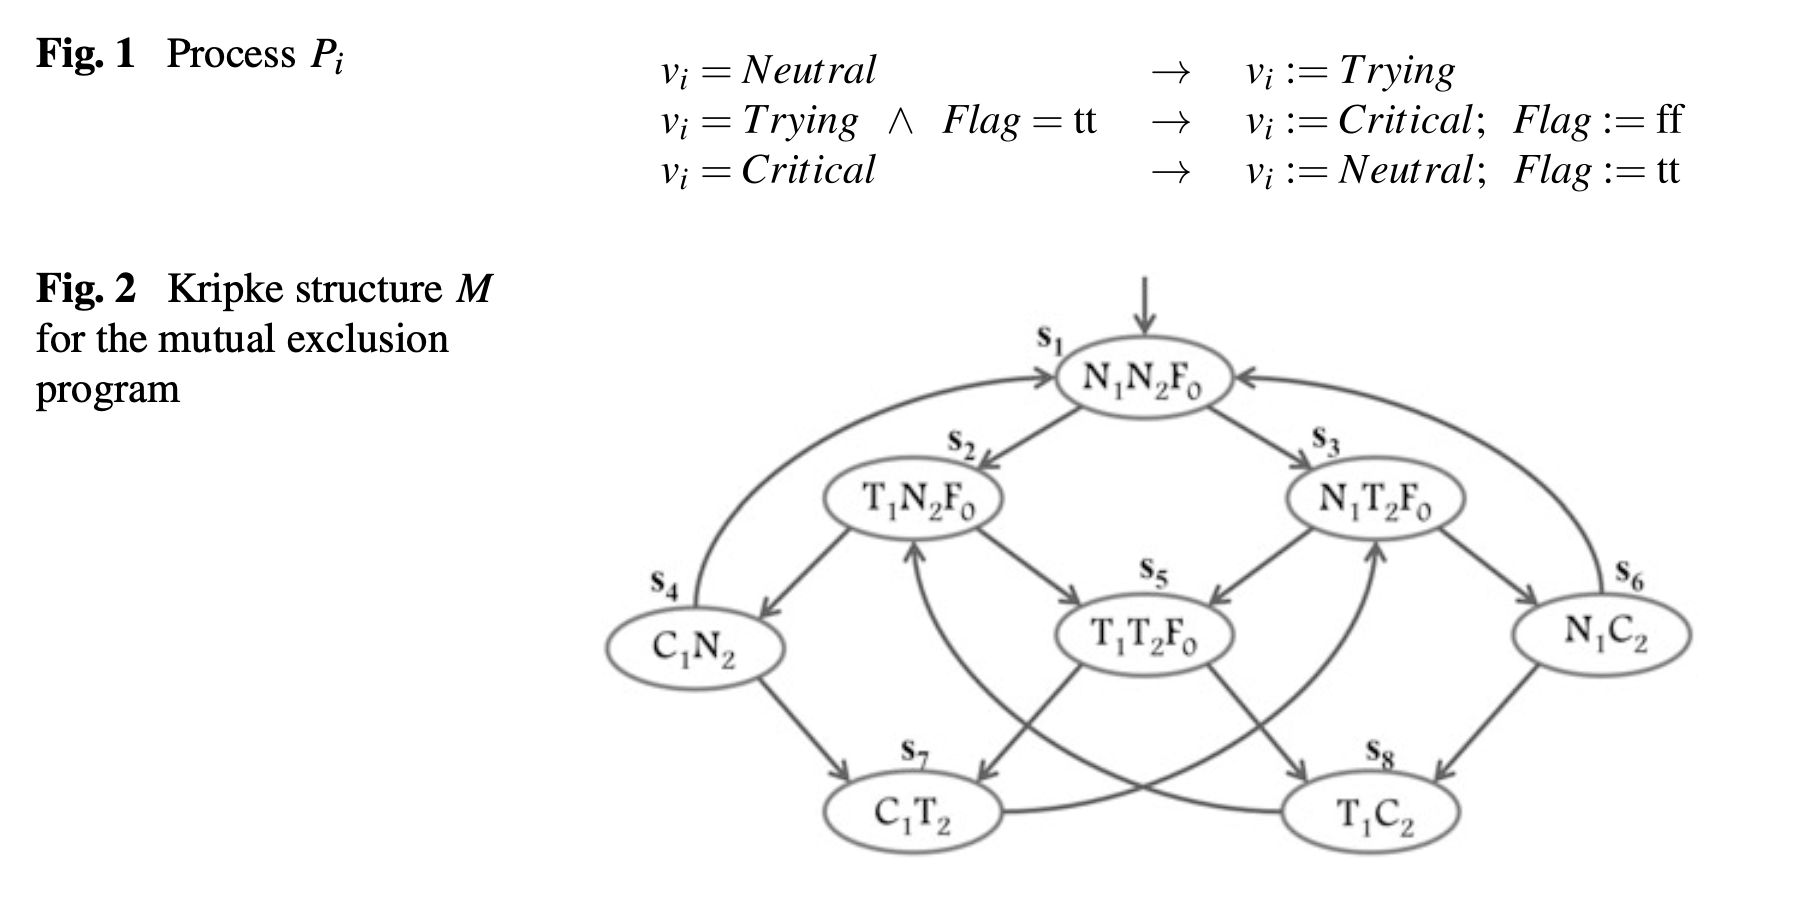
\includegraphics[scale=0.35]{images/concrete-mutex.png}
\end{center}
and then an abstraction of this structure, $M_1$, with atomic propositions $AP_1=\{C_1,C_2,F_0\}$:
\begin{center}
    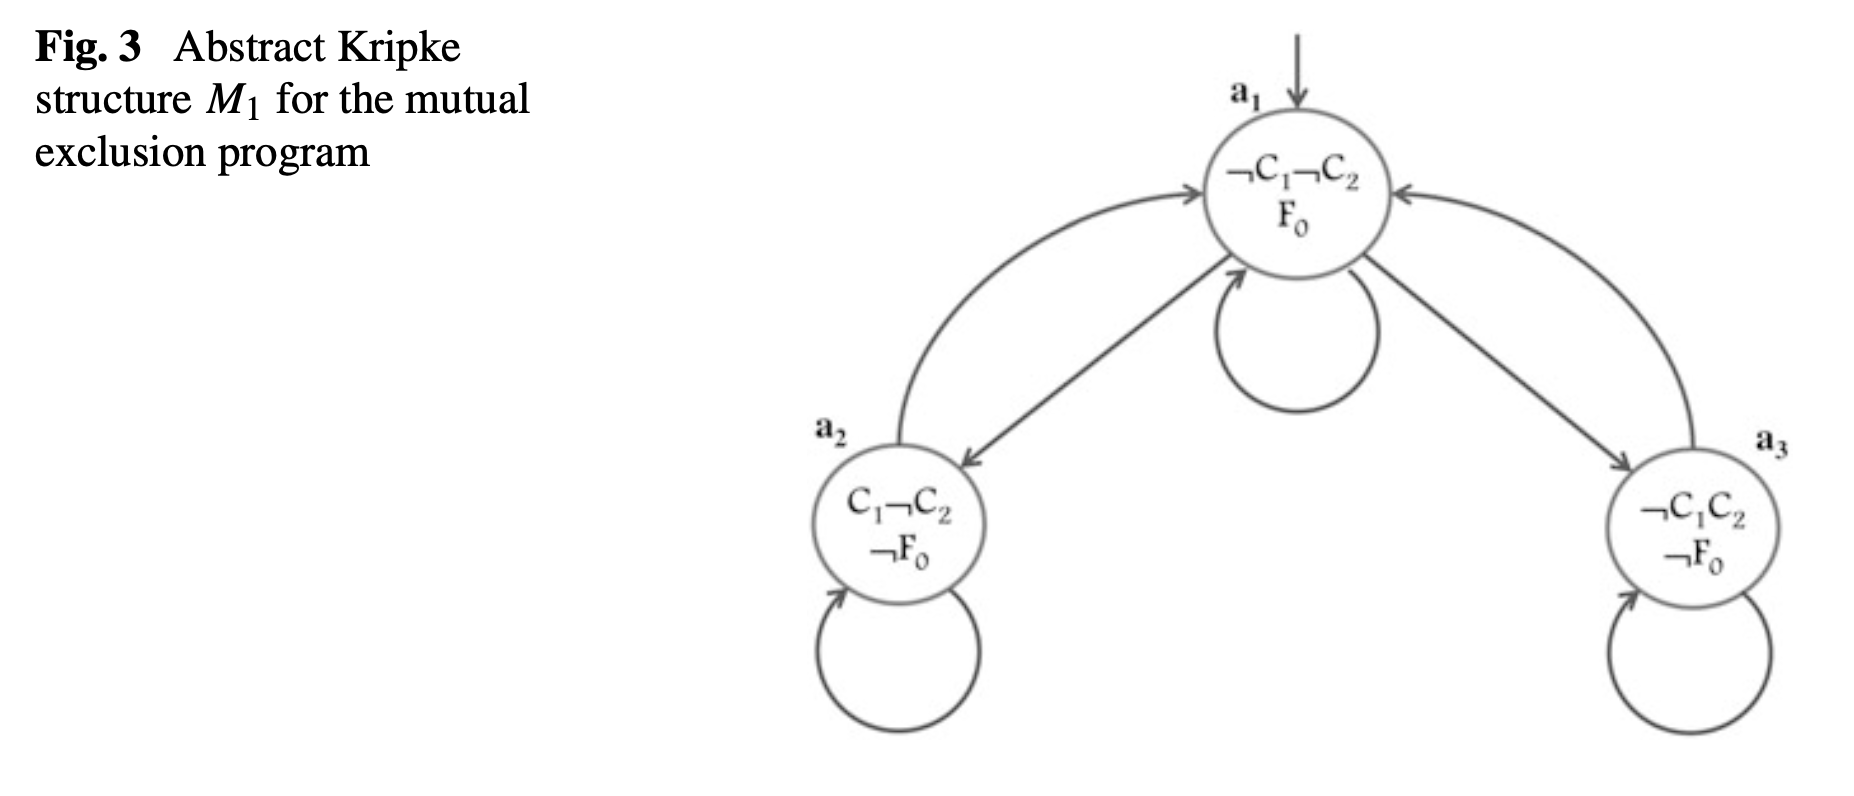
\includegraphics[scale=0.35]{images/abstract-mutex.png}
\end{center}
This abstraction basically only tracks whether a particular process is in the critical section or not, but ignores all other information. Note that $AP_1 \subseteq AP$. A simulation relation $H \subseteq S \times S_1$ from $M$ to $M_1$ can then be defined as 
\begin{align*}
    H = \left\lbrace (s_1, a_1), (s_2, a_1), (s_3, a_1), (s_4, a_2), (s_5, a_1), (s_6, a_3), (s_7, a_2), (s_8, a_3) \right\rbrace
\end{align*}

\subsubsection*{Bisimulation}

One state is related to another by the bisimulation relation If they agree on their common atomic propositions and, in addition, for every successor of one state there is a corresponding successor of the other state, and \textit{vice versa}.

\subsubsection*{Existential Abstraction}

One way to define an abstract model (Kripke structure) from a concrete one is via a concretization function $\gamma$. We can define abstract Kripke structures by means of \textit{existential abstraction} \cite{94mcabs}. Given a set $\widehat{S}$ of abstract states, the \textit{concretization function} $\gamma : \widehat{S} \rightarrow 2^S$ indicates, for each abstract state $\widehat{s}$, what set of concrete states are represented by $\widehat{s}$. Similarly, there is a transition from abstract state $\widehat{s}$ to another abstract state $\widehat{s}'$ if there is a transition from a state represented by $\widehat{s}$ to a state represented by $\widehat{s}'$. Essentially, we just take every transition between concrete states and add it into our abstract transition system, based on the abstract states that represent those concrete state transitions.

\subsubsection*{Trace Equivalence vs. Bisimulation}

Note that trace inclusion and trace equivalence notions of transition system similiarity or equivalence are often sufficient when concerned with linear time properties (i.e. LTL formulae)  \cite{2008principlemc}. Bisimulation and simulation can be considered primarily as relations that respect the \textit{branching time} behavior. Bisimulation, for example, is a stronger notion than trace equivalence. That is, if two systems $TS_1$ and $TS_2$ are bisimilar, then they admit the same set of traces. And so, these systems also fulfill the same linear time properties. 

\subsection*{Counterexample-Guided Abstraction Refinement (CEGAR)}


Regardless of how we choose our abstraction, our abstract model $\widehat{M}$ generally contains less information than the concrete model $M$, and so model checking $\widehat{M}$ may produce incorrect results. If a universal property is true in $\widehat{M}$ then it is also true in $M$, but if the abstract model produces an error, the concrete model may still be correct.

For example consider the following ``traffic light'' model and a simple abstraction of it
\begin{center}
    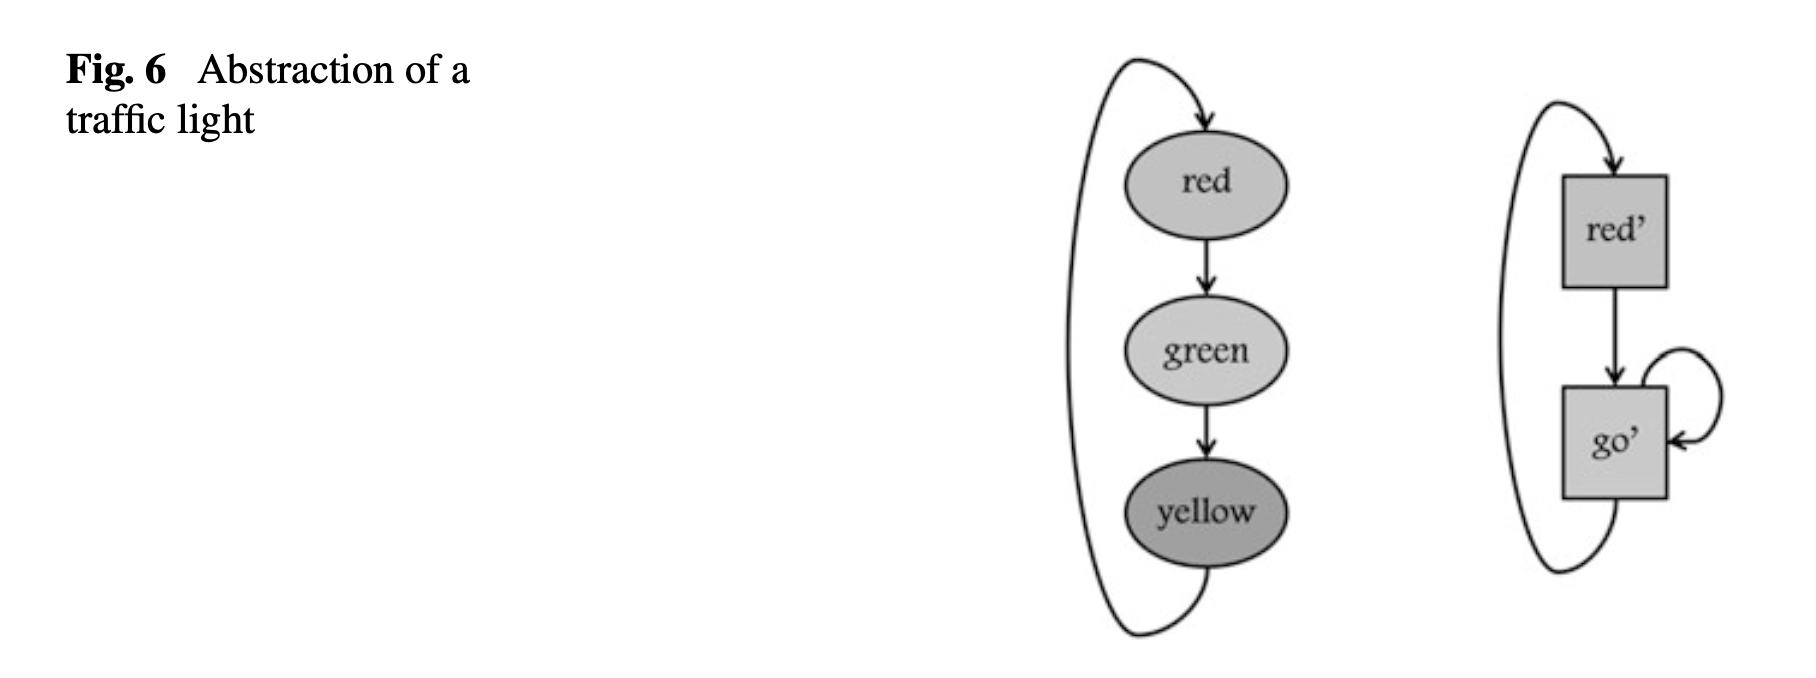
\includegraphics[scale=0.35]{images/cegar1.png}
\end{center}
If we wanted to check the universal CTL property $\textbf{AGAF}(IsRed)$ (i.e. along all paths, $IsRed$ holds infinitely often), this clearly holds in the concrete traffic light model, but fails in the abstract model. When an abstract counterexample does not correspond to any concrete counterexample, we call it \textit{spurious}.

Consider another example of a spurious counterexample, shown as follows:
\begin{center}
    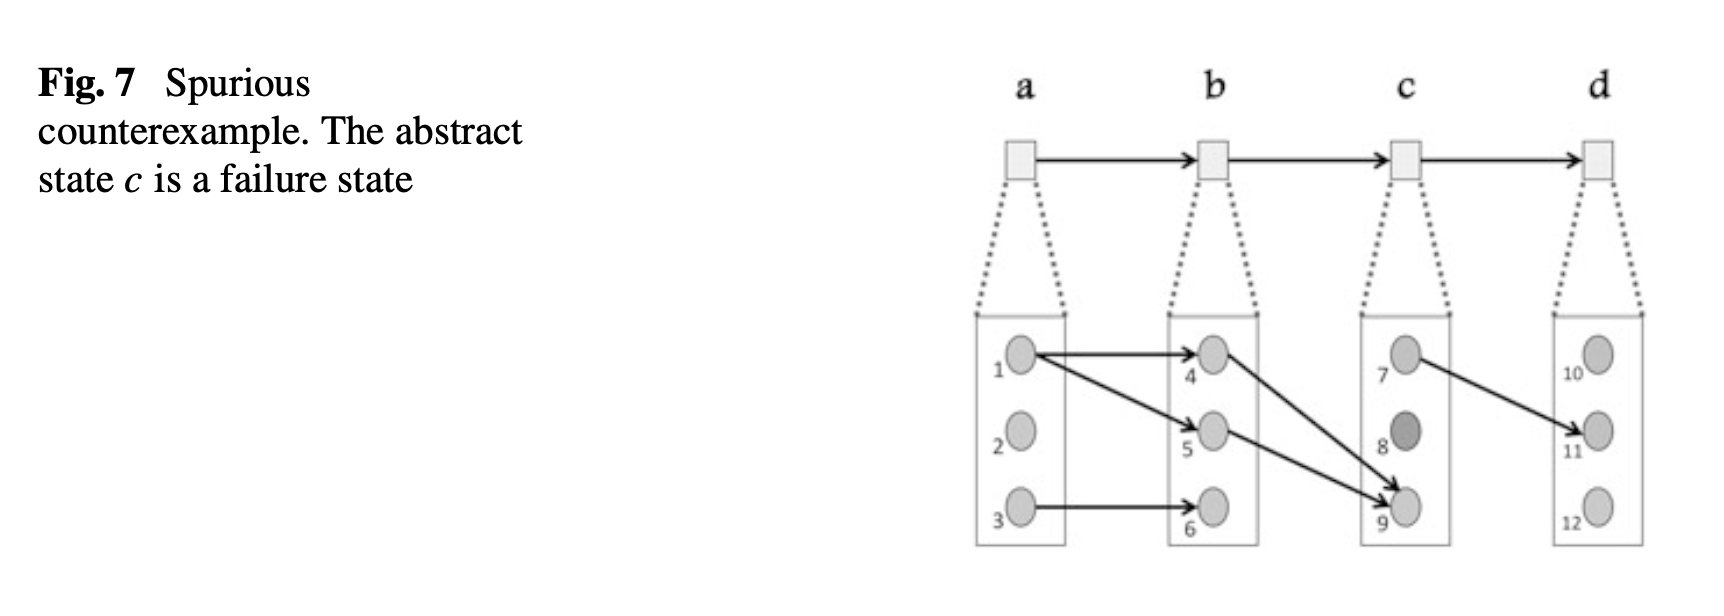
\includegraphics[scale=0.40]{images/cegar2.png}
\end{center}
in this case, reachability of state 11 is not preserved by the abstraction. That is, it is not reachable in the lower level system, but it is reachable in the abstract system (consisting of abstract states $\{a,b,c,d\}$).

The framework of \textit{counterexample-guided abstraction refinement (CEGAR)} deals with this issue. The main steps of CEGAR are as follows:
\begin{enumerate}
    \item Given a concrete model $M$ and some universal temporal formula to check, $\psi$, generate an initial abstract model $\widehat{M}$.
    \item Model check $\widehat{M}$ with respect to $\psi$. If $\widehat{M}$ satisfies $\psi$, then conclude that the concrete model satisfies $\psi$ and terminate. If a counterexample $\widehat{T}$ is found, check whether it is also a counterexample in the concrete model. 
    
    \begin{itemize}
        \item If it is, conclude that the concrete model does not satisfy the formula and stop.
        \item Otherwise, the counterexample is spurious, and proceed to step 3.
    \end{itemize}
    \item Refine the abstract model, $\widehat{M}$, so that $\widehat{T}$ will not be included in the new, refined abstract model. Go back to step 2.
\end{enumerate}

Note that refinement is typically done by \textit{partitioning} an abstract state. That is, the set of concrete states represented by the abstract state is partitioned

\subsubsection*{Identifying Spurious Counterexamples}

If we discover an abstract counterexample $\widehat{T}$, we need some way to check if this is a real counterexample in the concrete model. Assume that $\widehat{T}$ is a path $\widehat{s_1},\dots, \widehat{s_n}$ starting at the initial abstract state $\widehat{s_1}$. We can extend the concretization function $\gamma$ to sequences of abstract states as follows: $\gamma(\widehat{T})$ is the set of concrete paths defined as:
\begin{align*}
    \gamma(\widehat{T}) = \left\lbrace \langle s_1,\dots,s_n \rangle \mid 
    \bigwedge_{i=1}^n s_i \in \gamma(\widehat{s_i}) \wedge I(s_1) \wedge 
    \bigwedge_{i=1}^n R(s_i,s_{i+1})
    \right\rbrace
\end{align*}
Then, we need an algorithm to compute a sequence of sets of states that correspond to $\gamma({\widehat{T}})$. We let $S_1 = \gamma(\widehat{s_1}) \cap I$, and then define 
\begin{align*}
    S_i := Image(S_{i-1}, R) \cap \gamma(\widehat{s_i})
\end{align*}
where $Image(S_{i-1}, R)$ is the set of successors, in $M$, of the states in $S_{i-1}$. Basically, we just want to symbolically execute concrete model, starting from the concretized version of the initial abstract counterexample state, and, at each step, check whether there is some concrete state in this image set that corresponds to the set of states from the abstract counterexample. We can formalize this into the following lemma. Specifically, the following are equivalent:
\begin{enumerate}
    \item The path $\widehat{T}$ corresponds to a concrete counterexample.
    \item The set $\gamma(\widehat{T})$ of concrete paths is non-empty.
    \item For all $1 \leq i \leq n, S_i \neq \emptyset$.
\end{enumerate}

Note that checking whether a counterexample is spurious involves computations on the concrete model.

% If we start with some abstraction of our Kripke strucutre and try to model check it, we may encounter spurious errors. So, we use such a counterexample to refine our abstraction, and then repreat this process.

\subsection*{SAT-based Abstraction}

An alternative to the CEGAR based approach (introduced shortly after the initial CEGAR publication) is to rely more directly on a SAT solver for performing abstraction. A main idea is to do bounded model checking and then use proofs of unsatisfiability in this case to provide an \textit{explanation} of correctness, and to help us generate an abstraction for proving a property in the unbounded case. Using such a proof to generate an abstraction is called \textit{proof-based abstraction} \cite{2003abswithoutcex}. 

In the initial work of \cite{2003abswithoutcex} (appeared in \textit{TACAS 2003}, April), verification of a system $M$ is done by performing bounded model checking of $M$ for  a fixed bound $k$. If an error is found for this bound, then we're done, since a counterexample has been found. Otherwise, the SAT solver can return a (resolution) proof of unsatisfiability. This proof is used to generate an abstraction, $M'$, of $M$ by seeing what clauses of the encoding of $M$ are actually used in the proof (see \cite{2003abswithoutcex} for details). Then, \textit{unbounded} model checking is performed on the abstract model $M'$, which should in theory now be much cheaper since $M'$ has been abstracted from $M$. If model checking determines that there are no error traces in $M'$, then we are done. Otherwise, if model checking determines that $M'$ does have an error run, then we know its length $k'$ is greater than $k$. Thus, we then restart the procedure with $k'$ (or, generally, any value larger than $k'$)

\subsubsection*{Interpolation}

Slghtly subsequent work by McMillan \cite{2003satinterp} (appeared in \textit{CAV 2003}, July) presented an extension of this approach that makes use of \textit{interpolation} for doing abstraction with a SAT solver. Essentially this uses a similar bounded model checking approach and then extracts an \textit{interpolant} from a bounded unsatisfiability proof to compute an abstraction.

The standard bounded model checking unrolling is a constraint of the following basic form:
\begin{center}
    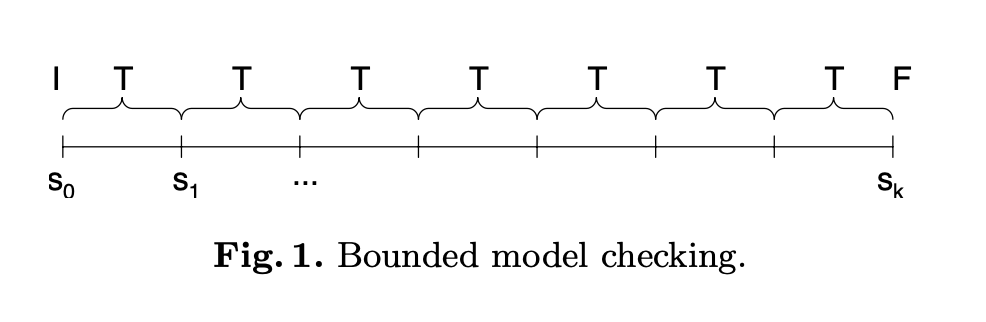
\includegraphics[scale=0.38]{images/bmc.png}
\end{center}
The idea of the interpolation based approach is to partition the path constraint into two sets $A$ and $B$:
\begin{center}
    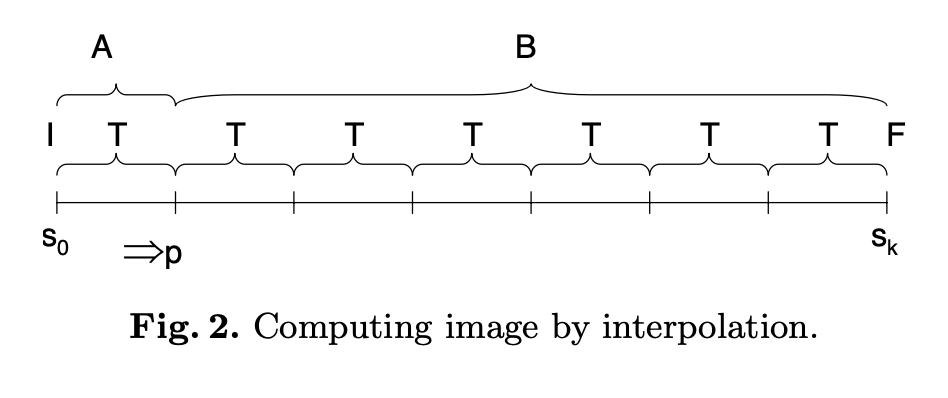
\includegraphics[scale=0.38]{images/bmc-interpolant.png}   
\end{center}
Then, if we produce a proof of unsatisfiability of the whole unrolling constraint, we derive an interpolant $P$ of the pair $(A,B)$, where the common variables of $A$ and $B$ are exactly those variables representing state $s_1$, in the sample diagram above. Note that an interpolant $P$ for two formulas $A,B$ is one such that 
\begin{itemize}
    \item $A \Rightarrow P$
    \item $P$ refers only to the common variables of $A$ and $B$
    \item $P \wedge B$ is unsatisfiable
\end{itemize}

By this, we can know that $P$ is implied by the initial condition and by the first transition constraint, so it represents some approximation of all 1-step reachable states (i.e. it is an over-approximation of the forward image of $I$). Moreover, $P$ and $B$ are unsatisfiable, meaning that no state satisfying $P$ can reach a final state in $k-1$ steps. This over-approximate image operation can then be iterated to compute an over-approximation of the reachable states. 

\begin{itemize}
    \item What is the difference between abstracting the entire system (e.g. the transition relation) and model checking that (like in CEGAR) vs. coming up with an abstraction of the reachable states and checking for inductiveness? Are these two approaches different but related in some way? Are there advantages to one over the other?
\end{itemize}

\bibliographystyle{alpha}
\bibliography{../../references.bib}

\end{document}